% \section{\clade{}: Abstention Under Family-Only Evidence}

% \subsection{Design}

% \paragraph{Questions.}
% We build 856 multiple-choice questions from indication and contraindication
% edges: 300 whose page names the answer, 256 whose page names only its family,
% and 300 whose page is silent (150 per relation and group, except 106 family-only
% contraindications, the most available). Each question offers five diseases and
% a sixth option, ``Not enough information to tell,'' labeled A to F. Wrong
% options come from the answer's MONDO neighborhood: its siblings first, then its
% cousins (the other grandchildren of its grandparent), and random diseases only
% when those run out. Neighbors exclude the answer's own ancestors and
% descendants and any other disease the drug is related to by the same
% relation. Most wrong options thus share the answer's family, so a family name
% eliminates few of them.

% \paragraph{Pages.}
% Each question is asked twice: once closed book and once with a passage from
% the drug's text, its cleaned Wikipedia article followed by its PubMed
% abstracts. The passage is the first 800 characters of that text plus a
% 280-character window on each side of every mention of the disease or its
% family, merged where windows overlap and capped at 1,800 characters; for
% silent questions it is therefore the opening of the text. Edges whose cleaned
% passage no longer shows the
% answer or family are replaced by other edges.

% \paragraph{Implementation.}
% All models run on CPU with Hugging Face Transformers. Prompts are scored in
% batches with left padding and explicit position indices. For the recovery
% experiment, the prompt prefix shared by all candidates is encoded once and
% reused; a sample of these scores is checked against a full forward pass
% before each run. Code and data splits will be released.

% \paragraph{Models and scoring.}
% We test five instruction-tuned models: Qwen2.5 0.5B, 7B and 14B
% \citep{qwen2025qwen25}, OLMo~2 7B \citep{olmo2024olmo2}, and Granite~3.1 8B
% \citep{granite2024}. The prompt lists the options, and the model's answer is
% the option letter with the highest next-token probability, renormalized over
% the six letters. A question is \emph{declined} when the model picks ``Not
% enough information.''

% \paragraph{Controls.}
% Two differences between the groups could produce a gap on their own. First,
% family-only questions more often have all four distractors from the
% neighborhood, which are harder to eliminate. We therefore analyze only such
% questions (106 named, 215 family-only and 160 silent).
% Second, the groups contain different facts, and some facts are harder than
% others even without a page. We therefore compare, for each question, its
% outcome with the page against its outcome closed book, and then compare this
% page effect between family-only and silent questions. The difference of these
% page effects is our main measure. Confidence intervals come from 5,000
% bootstrap resamples of questions. To pool across the three 7--8B models, we
% average each question's page effect over the models before comparing groups,
% so each question counts once. The supplementary material gives the passage
% and prompt formats, sampling details, formulas, queries and full result
% tables.

% \subsection{Results}

% \begin{table}[t]
% \centering
% \small
% \setlength{\tabcolsep}{3.2pt}
% \begin{tabular}{llcccc}
% \toprule
% Model & Page & Correct & Wrong & Declines & Prec. \\
% \midrule
% \multirow{3}{*}{Qwen2.5-7B} & named & 71.7 & 3.8 & 24.5 & 95.0 \\
%  & family & 26.5 & 18.1 & 55.3 & 59.4 \\
%  & silent & 13.8 & 2.5 & 83.8 & 84.6 \\
% \midrule
% \multirow{3}{*}{OLMo 2 7B} & named & 77.4 & 15.1 & 7.5 & 83.7 \\
%  & family & 37.2 & 44.7 & 18.1 & 45.5 \\
%  & silent & 30.6 & 24.4 & 45.0 & 55.7 \\
% \midrule
% \multirow{3}{*}{Granite 3.1 8B} & named & 72.6 & 7.5 & 19.8 & 90.6 \\
%  & family & 30.2 & 26.5 & 43.3 & 53.3 \\
%  & silent & 15.0 & 10.0 & 75.0 & 60.0 \\
% \midrule
% \multirow{3}{*}{Qwen2.5 0.5B} & named & 77.4 & 14.2 & 8.5 & 84.5 \\
%  & family & 34.4 & 55.8 & 9.8 & 38.1 \\
%  & silent & 28.7 & 50.6 & 20.6 & 36.2 \\
% \midrule
% \multirow{3}{*}{Qwen2.5 14B} & named & 67.9 & 2.8 & 29.2 & 96.0 \\
%  & family & 24.2 & 17.2 & 58.6 & 58.4 \\
%  & silent & 11.9 & 2.5 & 85.6 & 82.6 \\
% \bottomrule
% \end{tabular}
% \caption{Outcomes with the page (\%), questions whose four distractors all come from the answer's neighborhood
% (106 named, 215 family-only, 160 silent). Precision is the share correct among
% questions the model answered.}
% \label{tab:outcomes}
% \end{table}

% \begin{figure*}[t]
% \centering
% 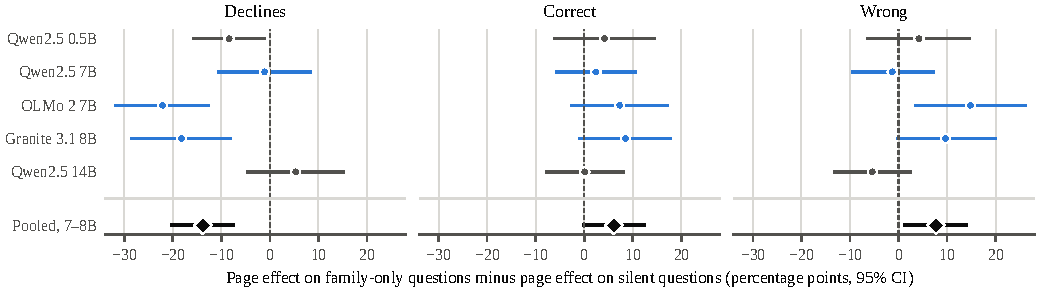
\includegraphics[width=\textwidth]{fig_forest.pdf}
% \caption{What a family-only page does, relative to a silent page. For each
% question, the page effect is its outcome with the page minus its outcome
% closed book; the plot shows the mean page effect on family-only questions
% minus that on silent questions, with 95\% bootstrap intervals. The pooled row
% averages each question over the three 7--8B models (481 questions). Gray rows
% are outside the pooled set.}
% \label{fig:forest}
% \end{figure*}

% \paragraph{With the page in hand, models decline less when it names only the
% family.}
% Table~\ref{tab:outcomes} gives outcomes with the page. In all three 7--8B
% models, a family-only page leads to fewer declines than a silent page: 55.3\%
% against 83.8\% for Qwen2.5-7B, 18.1\% against 45.0\% for OLMo~2, and 43.3\%
% against 75.0\% for Granite. The model answers more, and it answers less
% precisely: among answered questions, family-only pages give 45.5--59.4\%
% precision, against 83.7--95.0\% for pages that name the disease.


% \paragraph{The effect is the page's, not the questions'.}
% The raw comparison also reflects differences between the facts in each group.
% With no page, family-only questions already produce more wrong answers than
% silent ones in all three models (32.6\% against 15.6\% for Qwen2.5-7B, 56.7\%
% against 51.2\% for OLMo~2, 33.0\% against 26.2\% for Granite; supplement), so part of the gap in Table~\ref{tab:outcomes} comes from which facts
% fall in which group. Figure~\ref{fig:forest} removes this by comparing each
% question with itself. Pooled over the three
% 7--8B models, a page raises declines by 14.7 points on family-only questions
% and by 28.5 points on silent ones, a difference of 13.8 points (95\% CI
% $-20.3$ to $-7.5$, $p = 3.6\times10^{-5}$), which holds after a Bonferroni
% correction for the three outcomes ($p = 1.1\times10^{-4}$). The freed
% answers split about evenly. A page lowers wrong answers by 11.0 points on
% family-only questions and by 18.8 on silent ones, a difference of 7.7 points
% (95\% CI 1.2 to 14.0, $p = 0.019$; 0.056 after correction), and it lowers
% correct answers by 3.7 and 9.8 points, a difference of 6.1 points (95\% CI
% $-0.1$ to 12.4, $p = 0.058$). The decline effect is individually significant
% for OLMo~2 ($-22.1$ points, $p = 6\times10^{-6}$) and Granite ($-18.2$ points,
% $p = 0.0006$). Qwen2.5-7B shows no difference in its page effect ($-1.1$
% points, $p = 0.82$): it already declines family-only questions less often
% without a page (32.1\% against 59.4\%), and the page
% raises declines by the same amount in both groups.

% \paragraph{Robustness.}
% The raw pattern holds for both relations in all three models (per-relation
% rates in the supplement), and the 0.5B model shows the decline effect as well
% ($-8.4$ points, 95\% CI $-15.7$ to $-1.1$, $p = 0.027$).

% The decline effect depends on how large the named family is. Splitting the
% family-only questions into thirds by the number of members, the pooled effect is
% $-17.3$ points (95\% CI $-26.2$ to $-8.2$) for families of up to 10 members
% and $-18.4$ ($-26.6$ to $-10.3$) for 11--20 members, but only $-6.5$
% ($-15.7$ to $+3.0$) for larger families (Figure~\ref{fig:fixes}c). A narrow
% family makes the page look answerable.

% \subsection{The Family Name Causes \clade{}}

% \begin{figure}[t]
% \centering
% 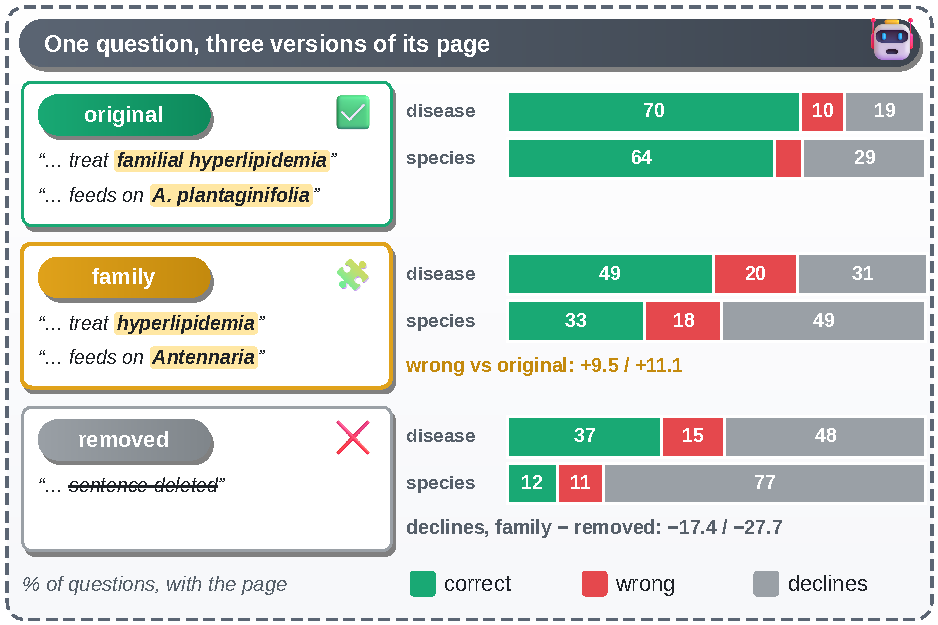
\includegraphics[width=\columnwidth]{fig_edit.pdf}
% \caption{Counterfactual page edit on the same named questions, for diseases
% (PrimeKG, 130 questions) and species (GloBI, 255). \emph{Family} replaces every
% mention of the answer with its parent; \emph{removed} deletes the sentences
% that mention it. Outcomes with the page (\%), averaged over three 7--8B
% models.}
% \label{fig:edit}
% \end{figure}

% The comparison above is between different facts. To hold the fact fixed, we
% edit the page itself. For the 130 named questions whose answer has a parent in
% MONDO, we build two versions of each page: \emph{family} replaces every mention
% of the answer with its parent's name, and \emph{removed} deletes the sentences
% that mention it. Question, options and model are unchanged; only the page
% differs.

% Figure~\ref{fig:edit} shows the result. Relative to the original page, the
% family version lowers correct answers by 21.0 points (95\% CI $-26.9$ to
% $-15.6$) and raises wrong answers by 9.5 (5.9 to 13.6), while declines rise by
% only 11.5 (7.4 to 15.9). Relative to deleting the mention, keeping the family
% name lowers declines by 17.4 points ($-23.6$ to $-11.5$) and raises both wrong
% answers, by 5.1 points (0.5 to 10.3), and correct ones, by 12.3 (6.9 to
% 17.9). Each model shows the same order: Qwen2.5-7B declines 70.0\% of the
% removed versions and 43.8\% of the family versions, Granite 56.2\% and
% 40.8\%, OLMo~2 18.5\% and 7.7\%. The family name therefore produces both
% effects seen in the observational comparison: it suppresses declining, and the
% answers it frees split between right and wrong.

% \subsection{Three Easy Fixes Leave \clade{} in Place}

% \begin{figure*}[t]
% \centering
% 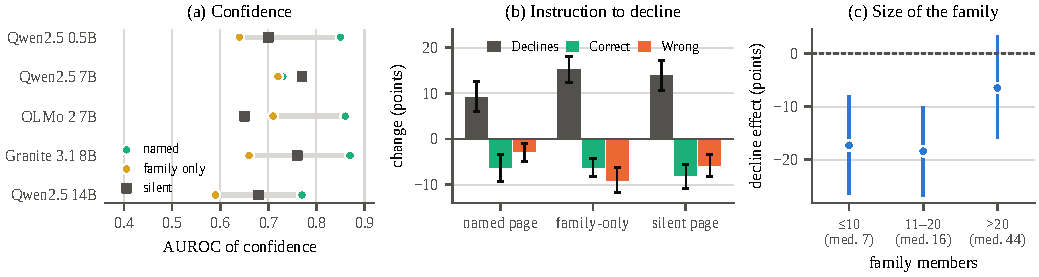
\includegraphics[width=\textwidth]{fig_fixes.pdf}
% \caption{Three easy fixes. (a) Confidence separates right from wrong answers
% less well on family-only pages in every model. (b) An instruction to decline
% when the page names only a broad category raises declines on every kind of page
% (pooled over three 7--8B models, 95\% CIs). (c) The decline effect of a
% family-only page is concentrated in small and medium families.}
% \label{fig:fixes}
% \end{figure*}


% \paragraph{Confidence does not flag these answers.}
% A system could answer only when the model is confident. Figure~\ref{fig:fixes}a
% shows that confidence separates right from wrong answers less well on
% family-only pages than on named pages in every model (AUROC 0.59--0.72 against
% 0.73--0.87). The wrong answers are confident: the mean probability of a wrong
% choice on a family-only page is 0.77--0.99 for the 7B and larger models, and
% 0.99 for Qwen2.5 14B. A threshold that keeps most correct answers keeps most of
% these wrong ones too.

% \paragraph{Scale does not remove the gap.}
% Qwen2.5 14B is more precise on named pages than any smaller model (96.0\%,
% Table~\ref{tab:outcomes}), but on family-only pages its precision stays at
% 58.4\%, and it gives 14.7 more points of wrong answers on family-only pages than
% on silent ones ($p = 6\times10^{-6}$). Like Qwen2.5-7B, it already declines
% family-only questions less often without a page, and its page effect does not
% differ between the groups ($+5.3$ points, $p = 0.29$).


% \paragraph{An instruction to decline is not targeted.}
% The simplest remedy is to tell the model: if the page names only a broad
% category that contains the answer, choose ``Not enough information.''
% Figure~\ref{fig:fixes}b shows that the instruction raises declines on
% family-only pages by 15.2 points (95\% CI 12.4 to 18.1), but also by 14.0 on silent pages and by 9.1
% on pages that name the answer, where it costs 6.3 points of correct answers
% ($-9.4$ to $-3.5$).
% Precision on family-only pages stays at 47.9--64.9\% after the instruction,
% far below the 89.6--94.7\% the same prompt gives on named pages (per-model
% rates in the supplement). The instruction does not help because the models do
% not tell a family name from an answer.

% \paragraph{What the result means.}
% A silent page pushes a model toward ``not enough information''; a page naming
% only the family pushes it much less, because it is relevant. The answers this
% frees are about as often wrong as right: the family name lets the model guess
% within a smaller space without telling it which member is meant, and a system
% that treats a relevant page as permission to answer will do so at 45--59\%
% precision while citing a relevant source.

% \subsection{\clade{} in a Second Domain: Species Interactions}

% \begin{table}[t]
% \centering
% \footnotesize
% \setlength{\tabcolsep}{3pt}
% \begin{tabular}{lrr}
% \toprule
%  & PrimeKG & GloBI \\
% \midrule
% Questions, pooled (all-sibling) & 481 & 833 \\
% Decline effect, family $-$ silent & $-13.8$ & $-14.3$ \\
% Wrong effect, family $-$ silent & $+7.7$ & $+11.6$ \\
% Precision, named page (\%) & 84--95 & 84--95 \\
% Precision, family-only page (\%) & 45--59 & 22--28 \\
% AUROC, named page & .73--.87 & .82--.86 \\
% AUROC, family-only page & .66--.72 & .52--.68 \\
% Edit: declines, family $-$ removed & $-17.4$ & $-27.7$ \\
% Edit: wrong, family $-$ removed & $+5.1$ & $+6.7$ \\
% Edit: correct, family $-$ original & $-21.0$ & $-30.8$ \\
% \bottomrule
% \end{tabular}
% \caption{The same tests on drug--disease facts (PrimeKG, MONDO) and on
% species interactions (GloBI, taxonomy), for the three 7--8B models. Effects
% in points; ranges are over models. All effects shown have 95\% CIs that
% exclude zero.}
% \label{tab:globi}
% \end{table}

% To test whether the effect depends on medicine or on MONDO, we repeat the
% abstention test and the counterfactual edit on species interactions from
% GloBI \citep{poelen2014globi}. We keep four relations (\emph{eats},
% \emph{preys on}, \emph{parasite of}, \emph{pollinates}) between species,
% use the consumer's Wikipedia article as the page, and use GloBI's taxonomy
% (species, genus, family) in place of MONDO. A page is named if it gives the
% partner's binomial, its abbreviated form or a common name from Wikipedia
% redirects, and family-only if it gives only the genus or family. Wrong options
% are species of the same genus, then of the same family, and never a recorded
% partner. The question set has 75 questions per group and relation (900 in all).

% Exact partners are rarely written down: of 23,694 measured edges, the page
% names the partner species for 3.9\% and only its genus or family for 7.1\%.
% Table~\ref{tab:globi} shows that every result carries over. A page raises
% declines by 12.1 points on silent questions but lowers them by 2.3 on
% family-only ones, a difference of $-14.3$ points ($p = 1.4\times10^{-9}$);
% the freed answers are mostly wrong ($+11.6$ points, $p = 2.5\times10^{-8}$;
% correct $+2.7$, $p = 0.09$). Family-only precision falls to 22--28\%, since
% species of one genus are harder to tell apart than diseases of one family. The
% counterfactual edit is stronger than on PrimeKG: keeping the genus name instead
% of deleting the sentence lowers declines by 27.7 points ($-32.2$ to $-23.5$)
% and raises wrong answers by 6.7 (3.4 to 10.2; Figure~\ref{fig:edit}). Resolvable insufficiency is a
% property of how text names facts that sit in a hierarchy, not of one domain.


% \section{Methodology}

% Our experimental methodology consists of four parts: (1) evaluating how coarse, family-only passages affect model abstention compared to silent and named passages; (2) performing counterfactual edits on passages to isolate the causal effect of the coarse category name; (3) testing whether standard mitigation strategies prevent premature guessing; and (4) evaluating a three-step ontology pipeline designed to recover the fine-grained answer.

% \subsection{Abstention Evaluation Setup}

% \paragraph{Multiple-choice questions with an abstention option.}
% We construct 856 multiple-choice questions from PrimeKG indication and contraindication facts: 300 with a \emph{named} passage, 256 with a \emph{family-only} passage, and 300 with a \emph{silent} passage (150 per relation and group, except for family-only contraindications, where all 106 available facts are used). Each question presents five candidate diseases alongside a sixth abstention option, \emph{Not enough information to tell}, labeled A through F.

% To make sure the options require fine-grained discrimination, we draw incorrect disease options (distractors) from the true answer's local neighborhood in MONDO. We select sibling diseases first (sharing the same parent), then cousin diseases (sharing the same grandparent), and use random diseases only when siblings and cousins are exhausted. We exclude any ancestor or descendant of the true answer, as well as any other disease linked to the drug by the same relation. Because most distractors belong to the same disease family as the true answer, seeing only the coarse family name in the passage does not logically rule them out.

% \paragraph{Passage construction.}
% Every question is evaluated twice: once closed book (no passage) and once open book (with a retrieved passage). Each passage is built from the drug's cleaned Wikipedia article followed by its retrieved PubMed abstracts. We include the first 800 characters of the text plus a 280-character context window around every mention of the target disease or its family, merging overlapping windows and capping total length at 1,800 characters. For silent passages, which have no mentions, this procedure yields the opening section of the drug's article.

% \paragraph{Models and scoring.}
% We evaluate five instruction-tuned open-weight models across three model families and three parameter scales: Qwen2.5 (0.5B, 7B, and 14B; \citealt{qwen2025qwen25}), OLMo~2 7B \citep{olmo2024olmo2}, and Granite~3.1 8B \citep{granite2024}. Models receive the passage, question, and six options A--F, and we select the option letter with the highest next-token probability (renormalized over the six option letters). We record an outcome as \emph{declined} (abstained) whenever the model selects \emph{Not enough information to tell}.

% \paragraph{Controlling for distractor difficulty and baseline fact hardness.}
% Two potential confounders could bias a naive comparison across passage types. First, family-only questions more frequently have enough relatives in MONDO to fill all four distractor slots with close neighbors, making those questions naturally harder. To eliminate this confounder, our primary analysis restricts all groups to questions where all four distractors come from the answer's MONDO neighborhood (106 named, 215 family-only, and 160 silent questions; full-sample results on all 856 questions appear in the supplement and show the same patterns).

% Second, different passage groups contain different underlying facts, which may vary in baseline difficulty even before a passage is read. We remove this baseline difference using a within-question difference-in-differences design. For each question, we first compute its \emph{page effect}: the outcome when given the passage minus the outcome when asked closed book. We then compare the mean page effect on family-only questions against the mean page effect on silent questions. Confidence intervals are estimated via 5,000 bootstrap resamples at the question level. When pooling across the three 7--8B models, we average each question's page effect across the three models before comparing groups so that each question receives equal weight.

% \subsection{Counterfactual Page Edits and Mitigation Tests}

% \paragraph{Counterfactual text edits.}
% Even with within-question controls, observational groups still test different sets of facts. To hold the underlying question and fact completely constant, we take the 130 named questions whose target disease has a MONDO parent and create two edited versions of each passage:
% \begin{itemize}
% \item \textbf{Family edit:} Every mention of the specific target disease in the passage is replaced with the name of its immediate MONDO parent category.
% \item \textbf{Removed edit:} Every sentence mentioning the target disease is deleted from the passage.
% \end{itemize}
% The question, multiple-choice options, and model remain identical; only the passage text changes.

% \paragraph{Three candidate fixes.}
% We test three practical strategies that might curb \clade{}:
% \begin{enumerate}
% \item \emph{Confidence thresholding:} Using the model's renormalized probability for its chosen answer to filter out uncertain guesses, measured via the area under the ROC curve (AUROC) for separating correct from wrong answers.
% \item \emph{Model scaling:} Comparing Qwen2.5 across 0.5B, 7B, and 14B parameters to see whether larger models abstain appropriately on coarse passages.
% \item \emph{Explicit abstention prompting:} Adding a direct instruction to the prompt telling the model to select \emph{Not enough information to tell} whenever the passage mentions only a broad category rather than a specific disease.
% \end{enumerate}

% \paragraph{Cross-domain replication on GloBI.}
% We replicate both the observational abstention experiment and the counterfactual page-edit experiment on 900 species-interaction questions from GloBI (75 questions per passage type across four ecological relations). Distractors are drawn first from species within the same genus, and then from the same family.

% \subsection{Ontology-Guided Recovery Pipeline}

% To test whether a symbolic ontology can resolve coarse passages into exact answers, we evaluate 410 PrimeKG indication and contraindication facts whose combined Wikipedia and PubMed text mentions only the disease family. Because a single drug often treats or is contraindicated for multiple related diseases within the same family (an average of 2.47 true diseases per family list), we count a recovered candidate as correct if it matches any true disease linked to that drug under the target relation.

% We decompose ontology-based recovery into three stages:
% \begin{enumerate}
% \item \textbf{Identifying the family and listing candidates:} We compare an oracle \emph{given-family} list (which takes the narrowest MONDO ancestor mentioned in the text and expands its descendants up to two levels down, capped at 64 candidates) against an automated \emph{page-built} list (which extracts every MONDO parent category mentioned in the drug's Wikipedia article and takes the union of their descendants, marking lists over 64 candidates as too broad).
% \item \textbf{Scoring and selecting a candidate:} Within the candidate list, we compare five selection methods: (a) Qwen2.5-7B scoring candidates closed book; (b) Qwen2.5-7B scoring candidates with the passage in the prompt; (c) Wikipedia reverse lookup (checking whether the candidate disease's own Wikipedia article mentions the drug); (d) PubMed co-mention counts (the number of PubMed abstracts mentioning both the drug and the candidate disease alongside relation-specific keywords, both raw and normalized by the disease's total PubMed volume); and (e) a simple \emph{popularity prior} that picks the candidate disease with the highest total number of PubMed abstracts regardless of the drug.
% \item \textbf{Non-ontology baselines:} We compare against two baselines that do not use MONDO: a list of the same length containing the true answer mixed with random diseases, scored by the model either with or without the passage in the prompt. Paired accuracy differences are evaluated using McNemar's test \citep{mcnemar1947}.
% \end{enumerate}







\section{Methodology}

We run four experiments. We measure how family-only pages change abstention, edit pages to isolate the effect of the family name, test three common fixes, and test whether an ontology can recover the exact answer.

\subsection{Abstention Evaluation Setup}
\label{subsec:abstention}

\paragraph{Questions.}
We curate 856 multiple-choice questions from the PrimeKG indications and contraindications: 300 with a \emph{named} page, 256 with a \emph{family-only} page, and 300 with a \emph{silent} page. Each relation and group has 150 questions, except family-only contraindications, where only 106 facts exist. Each question has five candidate diseases and a sixth option, \emph{Not enough information to tell}. The four wrong options come from the answer's MONDO neighborhood: siblings first, then cousins, then random diseases only if both run out. We exclude the answer's ancestors and descendants and any other disease the drug has under the same relation. 

\paragraph{Pages.}
We ask each question twice: closed book and with a page. The page starts with the drug's cleaned Wikipedia article, followed by its PubMed abstracts. We keep the first 800 characters and a 280 character window around each mention of the answer or its family, merge overlapping windows, and cap the page at \num{1800} characters. A silent page has no mentions, so it is the article's opening.

\paragraph{Models and Scoring.}
We evaluate five instruction-tuned open-weight models from three families: Qwen2.5 0.5B, 7B and 14B \citep{qwen2025qwen25}, OLMo~2 7B \citep{olmo2024olmo2}, and Granite~3.1 8B \citep{granite2024}. The model sees the page, the question and options A--F. We take the letter with the highest next-token probability, renormalized over the six letters. Choosing \emph{Not enough information to tell} counts as a decline. As a format check, we also ask 120 matched questions with no options and score each generated answer by name matching.

\paragraph{Controls.}
Two differences between groups could bias the comparison. First, family-only answers more often have enough relatives to fill all four wrong options, which makes those questions harder. Our main analysis therefore keeps only questions whose four wrong options all come from the neighborhood: 106 named, 215 family-only and 160 silent. Appendix~D reports all 856 questions, with the same pattern.

Second, the groups hold different facts, which may differ in difficulty before any page is read. We therefore compare each question with itself. For a question $q$ and an outcome such as a decline, let $y_q^{\text{page}}=1$ if the outcome occurs when the model reads the page and $0$ otherwise, and let $y_q^{\text{closed}}$ be the same without the page. The \emph{page effect} of $q$ is $y_q^{\text{page}}-y_q^{\text{closed}}$. Our main measure is the difference in mean page effect between the family-only questions $F$ and the silent questions $S$:
{\setlength{\abovedisplayskip}{3pt}\setlength{\belowdisplayskip}{3pt}%
\begin{equation}
\Delta = \frac{1}{|F|}\sum_{q\in F}\bigl(y_q^{\text{page}}-y_q^{\text{closed}}\bigr) - \frac{1}{|S|}\sum_{q\in S}\bigl(y_q^{\text{page}}-y_q^{\text{closed}}\bigr).
\label{eq:did}
\end{equation}}
For declines, $\Delta<0$ means a family-only page pushes the model toward declining less than a silent page does. To pool the 7--8B models, we average each question's page effect over the models first, so each question counts once.

\paragraph{Statistics.}
Effects are in percentage points. Brackets give 95\% confidence intervals (CI) from 5,000 bootstrap resamples of questions; an interval that excludes \num{0} marks a reliable effect. $p$-values come from two-sided $z$-tests (Appendix~C).

\subsection{Counterfactual Evaluation}

\paragraph{Page edits.}
The groups in~\cref{subsec:abstention} test different facts. To hold the fact fixed, we take 130 named questions whose answer has a MONDO parent. Then we edit each page in two ways: \emph{family edit} replaces every mention of the answer with its parent's name, and \emph{removed edit} deletes every sentence that mentions the answer (\cref{fig:edit}). The question, options and model stay the same.

\paragraph{Simple fixes fail.}
We test three ways to curb \clade{}. \emph{Confidence filtering} uses the renormalized probability of the chosen option; we report the AUROC for separating correct from wrong answers. \emph{Scaling} compares Qwen2.5 at 0.5B, 7B and 14B. \emph{Instruction} adds a line to the prompt telling the model to choose \emph{Not enough information to tell} when the page names only a broad category.

\paragraph{Second domain.}
We repeat the main experiment and counterfactual edits on 900 GloBI questions: 75 per page type in each of four relations. Wrong options come from the same genus first, then the same family.

\subsection{Ontology Recovery}

We test recovery on 410 PrimeKG facts whose Wikipedia and PubMed text names only the disease family (Figure~\ref{fig:concept}). A drug often has several true diseases in a family (2.47 per list on average), so a pick counts as correct if it matches any of them. Recovery has three stages:

\begin{enumerate}
\item \textbf{Build the list.} The oracle \emph{given-family} list takes the narrowest MONDO ancestor named in the text and lists its descendants up to two levels down, capped at 64. The automatic \emph{page-built} list takes every MONDO parent named in the drug's Wikipedia article and joins their descendants; lists over 64 count as too broad. The \emph{model-chosen} list asks Qwen2.5-7B which of the families on the page (up to ten) holds the answer and expands only that one.
\item \textbf{Choose one.} We compare five options: (1) Qwen2.5-7B closed book, (2) Qwen2.5-7B with the page in the prompt, (3) a reverse lookup to check whether the candidate's own Wikipedia article names the drug, (4) PubMed co-mention counts with relation keywords, raw and normalized by the disease's PubMed volume, and (5) a \emph{popularity prior} that picks the disease with the most PubMed abstracts, ignoring the drug.
\item \textbf{Compare without ontology.} Two baselines replace the family list with a list of the same length that holds the answer plus random diseases, scored by the model with or without the page. We test paired differences with McNemar's test \citep{mcnemar1947}.
\end{enumerate}


